\section{Test}
Tutti i test sono stati eseguiti su una macchina con sistema operativo windows 10, un processore Intel Core i7 4750HQ a 2.0GHz e con 12Gb di RAM DDR3.\\
Per ogni dataset utilizzato abbiamo testato il nostro algoritmo tramite la classe \textbf{MainClass.java} descritto nel capitolo di implementazione, ricavando così i tempi impiegati dal nostro algoritmo su ciascun dataset, provando ogni possibile colonna come RHS e le restanti colonne come LHS.  \\
Per ogni dataset abbiamo testato tutte le combinazioni di attributi sull'RHS e sull'LHS ciascuna per 10 volte in modo da avere una stima più accurata dei tempi. Abbiamo diviso il tempo complessivo in più parti, il tempo impiegato per calcolare la matrice delle distanze, il tempo per il Feasibility ed il tempo per gli ultimi due step. Per un testing più approfondito sono stati effettuati dei test con l'utilizzo di un numero differente di thread. Dato l'hardware su cui sono stati testati i dataset è stato possibile effettuare test su un numero di thread che va da 1 a 7.\\
Mostreremo quelli che sono i test ritenuti rilevanti:
\begin{itemize}
	\item Test in sequenziale;
	\item Test con un numero di thread pari a 2;
	\item Test con un numero di core fisici massimi(thread pari a 3);
	\item Test con thread massimi (pari a 7).
\end{itemize}
\subsection{Dataset utilizzati}
Oltre ad una serie di dataset creati appositamente per verificare la correttezza di alcune operazioni, abbiamo prelevato una serie di dataset dal sito dell'Information Systems Group dell'Hasso-Plattner-Institut \cite{metanome}: un un gruppo di ricerca della suddetta Università tedesca che si occupa, tra le altre cose, di progettare algoritmi dedicati alla ricerca delle dipendenze funzionali. Su tale sito, oltre a poter consultare gli algoritmi sviluppati, è possibile accedere a tutti i dataset sui quali tali algoritmi sono stati testati corredati a varie informazioni (i.e. fonte, numeri di attributi, numero di righe, dipendenze funzionali trovate, dipendenze funzionali ordinate trovate ecc).\\
\begin{table}[H]
	\centering
	\begin{tabular}{lllll}
		Nome & Attributi & Righe & Dimensione \\
		\hline
		dataset & 4 & 7 & 118 B \\
		Bridges & 13  & 108 & 6 Kb\\
		balance-scale  & 5  & 624 & 7 Kb\\
		echocardiogram  & 13  & 131 & 6,1 Kb\\
	\end{tabular}
	\caption{Dataset utilizzati}
	\label{datasetUtilizzati}
\end{table}
\subsection{Risultati test sequenziale}
In questa fase di testing mostreremo i risultati ottenuti lavorando in \textbf{sequenziale}.
Nella seguente tabella sono mostrati i risultati ottenuti dai test sui dataset considerati.
\begin{table}[H]
	\centering
	\begin{tabular}{lllll}
		Dataset & DM & Feasibility & Minimality e GenRFD & RFD trovate \\
		\hline
		dataset& $0,0005s$ & $0,016s$ & $2,5s$ & 82 \\
		Bridges & $0,215s$  & $0,860s$ & $8000s$ & 62912 \\
		balance-scale  & $1s$  & $0,016s$ & $0,172$ & 1\\
		echocardiogram  & $0,300s$  & $0,850s$ & $700s$ & 236852\\
		\hline
	\end{tabular}
	\label{risultati}
	\caption{RFD scoperte corredate dai tempi impiegati dall'algoritmo per ogni dataset}
\end{table}
\subsection{Risultati test con due thread}
In questa fase di testing mostreremo i risultati ottenuti lavorando con \textbf{due thread}, sfruttando appieno così la potenza di due core fisici presenti sul nostro hardware.
Nella seguente tabella sono mostrati i risultati ottenuti dai test sui dataset considerati.
\begin{table}[H]
	\centering
	\begin{tabular}{lllll}
		Dataset & DM & Feasibility & Minimality e GenRFD & RFD trovate \\
		\hline
		dataset& $0,0005s$ & $0,002$ & $2s$ & 82 \\
		Bridges & $0,190s$  & $0,730s$ & $7400$ & 62912 \\
		balance-scale  & $900s$  & $0,016s$ & $0,125$ & 1\\
		echocardiogram  & $0,250s$  & $0,600s$ & $600s$ & 236852\\
		\hline
	\end{tabular}
	\label{risultati_2_thread}
	\caption{RFD scoperte corredate dai tempi impiegati dall'algoritmo per ogni dataset con due thread}
\end{table}
\subsection{Risultati test con tre thread}
Dopo aver visto gli effetti sul testing del multithreading tentiamo ora di sfruttare al meglio quelli che sono i core fisici del nostro processore allocandone \textbf{tre} per l'algoritmo.
Nella seguente tabella sono mostrati i risultati ottenuti dai test sui dataset considerati.
\begin{table}[H]
	\centering
	\begin{tabular}{lllll}
		Dataset & DM & Feasibility & Minimality e GenRFD & RFD trovate \\
		\hline
		dataset& $0,0005s$ & $0,002$ & $2s$ & 82 \\
		Bridges & $0,190s$  & $0,730s$ & $7200s$ & 62912 \\
		balance-scale  & $900s$  & $0,016s$ & $0,110$ & 1\\
		echocardiogram  & $0,250s$  & $0,570s$ & $570s$ & 236852\\
		\hline
	\end{tabular}
	\label{risultati_3_thread}
	\caption{RFD scoperte corredate dai tempi impiegati dall'algoritmo per ogni dataset con tre thread}
\end{table}
\subsection{Risultati test con sette thread}
Nell'ultima fase dei test effettuati andiamo a sfruttare al meglio la tecnologia in nostro possesso.
A questo punto andremo ad utilizzare l'\emph{hyperthreading}, cioè la virtualizzazione dei core fisici presenti sulla CPU. In questo caso utilizzeremo \textbf{sette thread}.
Nella seguente tabella sono mostrati i risultati ottenuti dai test sui dataset considerati.
\begin{table}[H]
	\centering
	\begin{tabular}{lllll}
		Dataset & DM & Feasibility & Minimality e GenRFD & RFD trovate \\
		\hline
		dataset& $0,0005s$ & $0,002s$& $2s$  & 82 \\
		Bridges & $0,190s$  & $0,730s$ & $6900$ & 62912 \\
		balance-scale  & $700s$  & $0,016s$ & $0,100$ & 1\\
		echocardiogram  & $0,220s$  & $0,510s$ & $550s$ & 236852\\
		\hline
	\end{tabular}
	\label{risultati_7_thread}
	\caption{RFD scoperte corredate dai tempi impiegati dall'algoritmo per ogni dataset con sette thread}
\end{table}
\subsection{Considerazioni finali su testing}
Da una prima osservazione possiamo notare come, rispetto a \textit{dataset}, \textit{Balance-scale} richieda molto più tempo per computare la matrice delle distanze. Questo è dovuto alla differenza sostanziale che esiste tra il numero di righe dei due dataset. 
Altra importante osservazione va effettuata sulla creazione degli \textbf{insiemiC} attuata durante il \emph{Feasibility}. Notiamo, infatti, che i dataset con una presenza maggiore di righe impieghino un tempo superiore rispetto a \emph{balance-scale} o \emph{dataset}.
Possiamo inoltre dare una piccola occhiata ai tempi per le ultime due fasi.
Da una prima osservazione notiamo come man mano che il numero di RFD aumenta, il tempo di esecuzione cresce sempre più velocemente. Ciò è dovuto alla natura non lineare dell'algoritmo, in particolare al notevole aumento del numero di iterazioni necessarie all'aumentare delle RFD scoperte.
Ora facciamo una piccola analisi che riguarda la parte multithreading del nostro algoritmo.
Possiamo notare che per algoritmi di piccole dimensioni, il fatto di utilizzare più thread porta un beneficio quasi nullo, anzi, in alcuni casi porta a delle piccole inflessioni delle prestazioni. Questo comportamento bizzarro è dovuto alla sincronizzazione applicata da \emph{AKKA} ai nostri thread. Siccome la mole di lavoro per ogni singolo thread è insignificante, allora il tempo maggiore viene impiegato per la gestione attraverso il container(\emph{Actor System}).
Il miglioramento invece lo si evince dai risultati ottenuti per dataset di dimensioni più grandi, come possiamo ben vedere con \emph{echocardiogram}.
\begin{figure}[H]
	\centering
	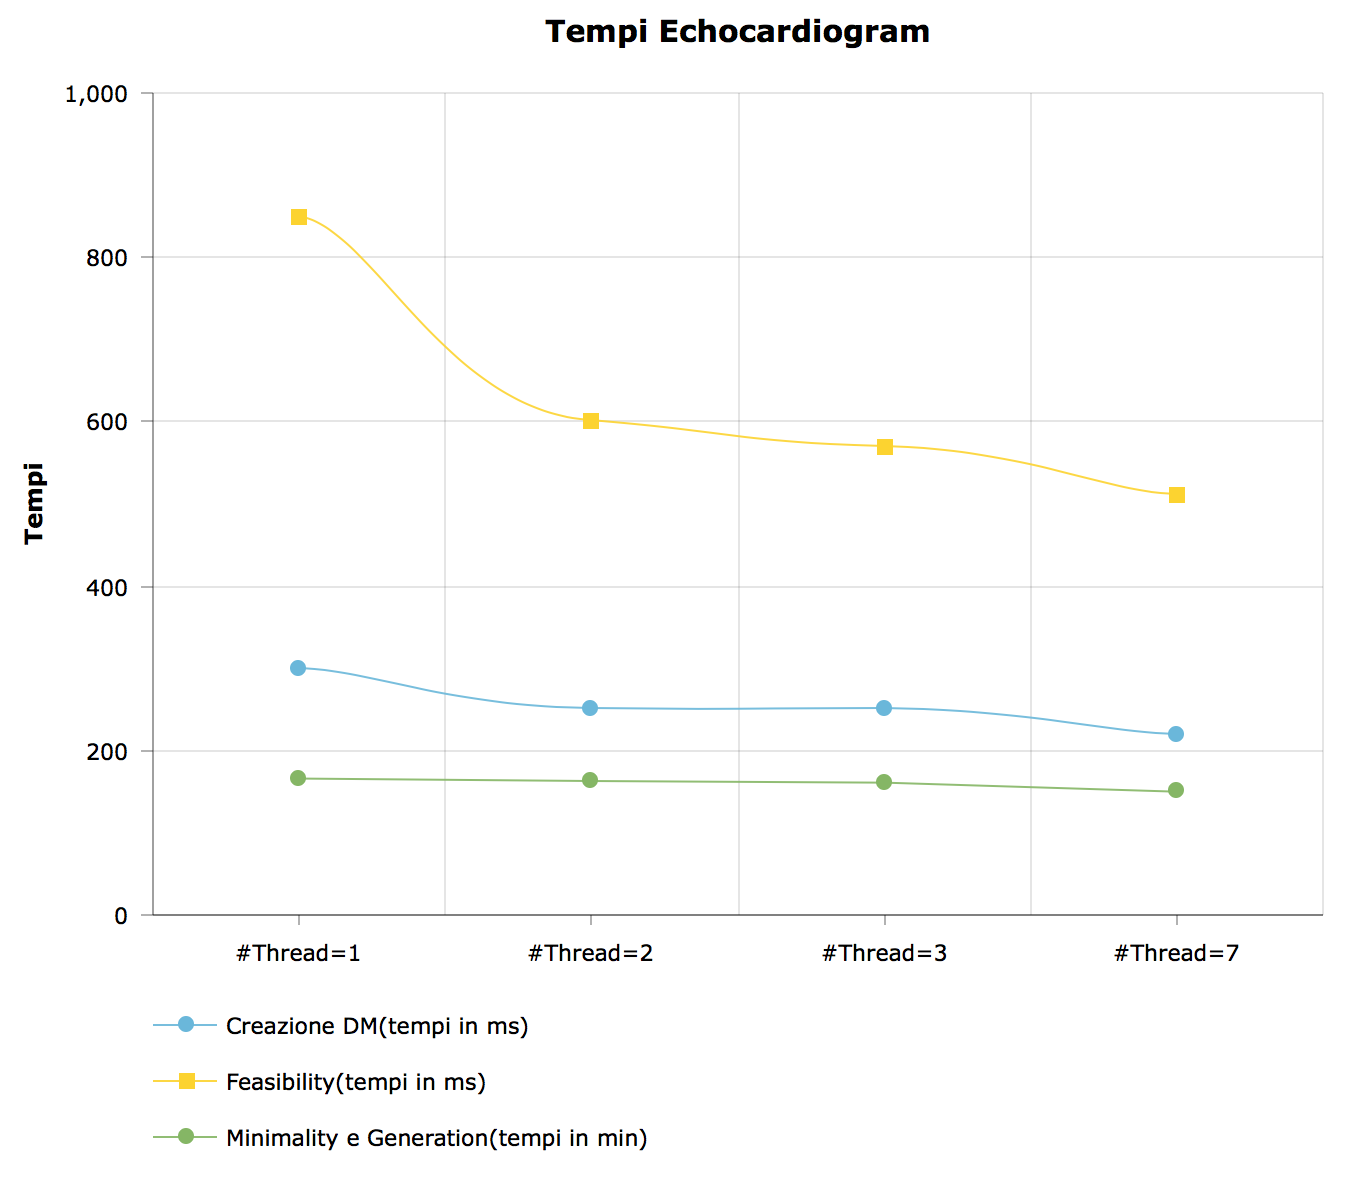
\includegraphics[scale = 0.4]{Immagini/GraficoEchocardiogram.png}
	\caption{Tempi ricerca RFD per Echocardiogram}
	\label{fig:tempi_Echocardiogram}
\end{figure}